
\chapter{Preliminaries}
\label{chap:prelims}
%%%%%%%%%%%%%%%%%%%%%%%%%%%%%%
% moved here from motivation section.
%%%%%%%%%%%%%%%%%%%%%%%%%%%%%%
\begin{figure*}[!ht]
  \centering
    \subfloat[Emulation ]{
      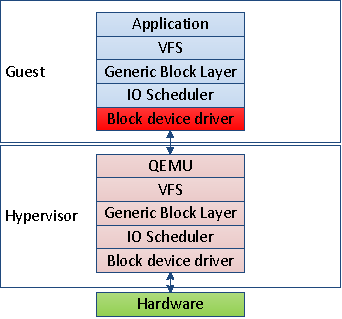
\includegraphics[width=0.3\textwidth]{figs/emulation.pdf}
      \label{fig:storage:emulation}
    }
    \hfill
    \subfloat[virtio]{
      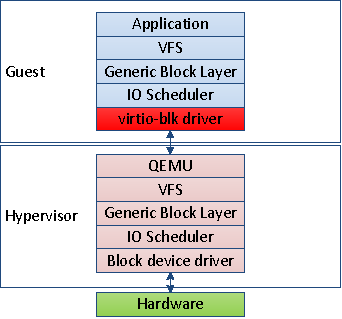
\includegraphics[width=0.3\textwidth]{figs/virtio.pdf}
      \label{fig:storage:virtio}
    }
    \hfill
    \subfloat[Direct-IO]{
      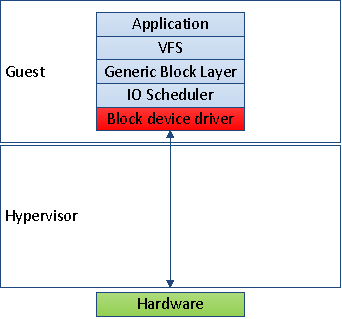
\includegraphics[width=0.3\textwidth]{figs/direct.pdf}
      \label{fig:storage:direct}
    }
    \caption{IO Virtualization techniques.
      \label{fig:storage}}
    
\end{figure*}
%%%%%%%%%%%%%%%%%%%%%%%%%%%%%%


Hypervisors virtualize local storage resources by mapping guest storage devices onto files in their local filesystem, in a method commonly referred to as a nested filesystem~\cite{le12nested}. As a result, they replicate the guest operating system's (OS) software layers that abstract and secure the storage devices. Notably, these software layers have been shown to present a performance bottleneck even when not replicated~\cite{yu14swoverheads}, due to the rapid increase in storage device bandwidth ~\cite{intel-ssd,seagate16ssd}.
%
Moreover, further performance degradation is caused by the method by which hypervisors virtualize storage devices and the resulting communication overheads between the guest OS and the underlying hypervisor.
Consequently, the storage system is becoming a major bottleneck in modern virtualized environments.
%
In this section we examine the sources of these overheads and outline how they can be mediated using a self-virtualizing storage device.

% software layers
Prevalent storage devices present the software stack with a raw array of logical block addresses (LBA), and it is up to the OS to provide a flexible method to partition the storage resources into logical objects, or files. In addition, the OS must enforce security policies to prevent applications from operating on data they are not allowed to operate on.
%
The main software layer that provides these functionalities is the filesystem, which combines both allocation and mapping strategies to construct logical objects and map them to physical blocks (for brevity, we focus the discussion on these two functionalities and ignore the plethora of other goals set by different filesystems). In addition, the filesystem layer also maintains protection and access permissions. Besides the filesystem, another common layer is the block layer, which caches disk blocks and abstracts the subtleties of different storage devices from the filesystem layer.

When an application accesses a file, the OS uses the filesystem layer to check the access permissions and map the file offset to an LBA on the storage device. It then accesses its block layer, which retrieves the block either from its caches or from the physical device. In a VM, this process is replicated since the storage device viewed by the guest OS is actually a virtual device that is mapped by the hypervisor to a file on the host's storage system. Consequently, the hypervisor invokes its own filesystem and block layers to retrieve the data to the guest OS. 

% virtualization method
Figure~\ref{fig:storage} illustrates the three most common methods by which hypervisors virtualize storage devices:


